%!TEX root = main.tex
% UTF-8 encoding
% \begin{figure*}[t]
% 	\centering
% 	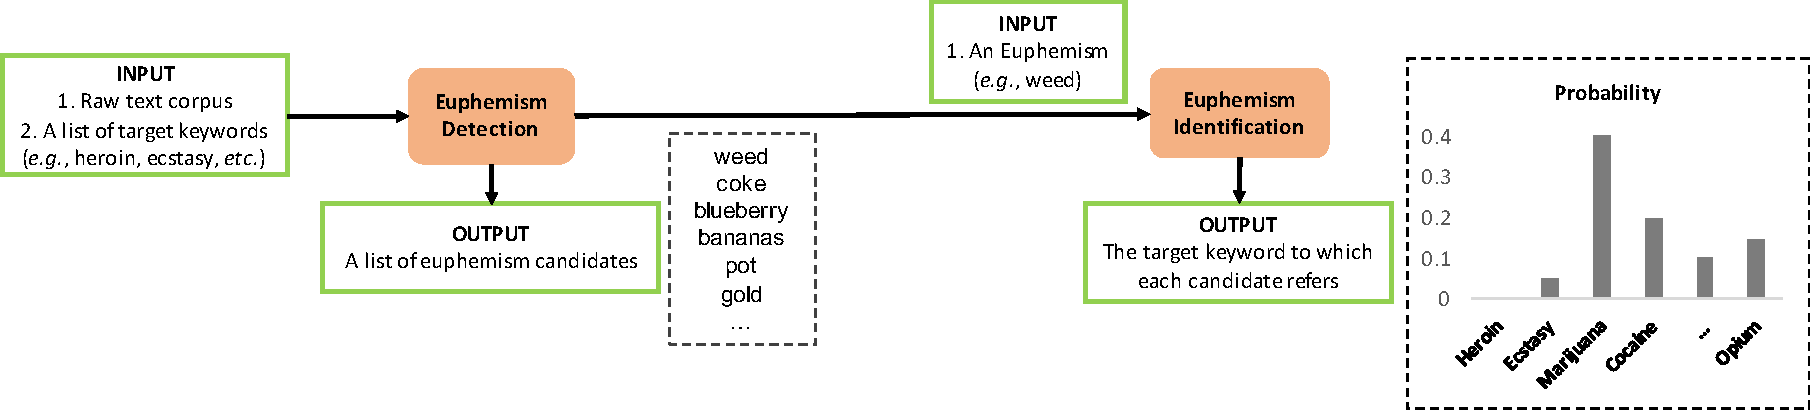
\includegraphics[width=0.98\linewidth]{figures/1}
% 	\caption{An overview of the task.}
% 	\label{fig:model_overview}
% \end{figure*}


\section{Problem Description}
\label{sec:problem}


In this study, we assume a content moderator that has access to a textual corpus (\eg, a set of posts from an online forum), 
and is required to moderate content related to a given list of target keywords. 
In practice, forum users may use \emph{euphemisms}---words that are used as substitutes for  one of the target keywords. 
We have two goals, euphemism detection and euphemism identification, defined as follows: 
1) \emph{Euphemism detection:} Learn which words are being used as euphemisms for keywords. A moderator can use this to filter content that may need to be moderated.
2) \emph{Euphemism identification:} Learn the meaning of euphemisms. This can be used by the moderator to understand context, and individually review content that uses euphemisms. 
% Our goal is to detect euphemisms in the corpus,   (\eg, a data dump from an online forum) and for each euphemism to identify the target keyword it refers to. 

As shown in Figure \ref{fig:model_overview}, these two tasks are complementary and form, together, a content moderation pipeline.
The euphemism detection task takes as input (a) the raw text corpus, and (b) a list of target keywords (\eg, heroin, marijuana, ecstasy, \etc). 
The expected output is an ordered ranked list of euphemism candidates, sorted by model confidence. 
% Once a euphemism is successfully detected, we are interested in identifying which target keyword it refers to, by a euphemism identification module. 
The euphemism identification module takes as input a euphemism (\eg, weed) and  outputs a probability distribution over the target keywords in the list. 
For example, if we feed the euphemism \emph{weed} into this module, the output should be a probability distribution over keywords, with most of the mass on \emph{marijuana}.
% Take ``weed'' as an example, we expect the identification module tells that it is more likely to be marijuana than other drugs. 


\noindent \textbf{Remark}: 
We use the term ``category'' to denote a 
topic (\ie, drug, weapon, sexuality). 
We use ``target keyword'' to refer to the specific keyword in each category users might be trying to use euphemisms for (\eg, ``marijuana'' and ``heroin'' are example of target keywords in the drug category). 
